\section{Exercises}

\begin{exercise}[\textbf{Computational Complexity}]
What is the computational complexity (per-iteration, in terms of $k$ -- the number of features) of LSTD and TD(0)? Suggest an improvement to the matrix-inversion step of LSTD to reduce the computational complexity (hint: use the Sherman Morrison formula).
\end{exercise}

\begin{exercise}[\textbf{Projected Bellman Operator}]
Consider the projection operator $\Pi $ that projects a vector $V\in \mathbb R^n$ to a linear subspace $S$ that is the span of $k$ features ${\phi _1}(s), \ldots ,{\phi _k}(s)$ w.r.t. the $\epsilon$-weighted Euclidean norm.
Also recall the Bellman operator for a fixed policy ${T^\pi }(v) \doteq r + \gamma {P^\pi }v$.

\begin{enumerate}
  \item Show that for a vector $v \in S$, the vector $v' = {T^\pi }v$ is not necessarily in $S$. Choose an appropriate MDP and features to show this.
\end{enumerate}

In class we have seen that $\Pi {T^\pi }$ is a contraction w.r.t. the  $\epsilon$-weighted Euclidean norm, when $\epsilon$ is the stationary distribution of ${P^\pi }$. We will now show that when $\epsilon$  is chosen differently, $\Pi {T^\pi }$ is not necessarily a contraction.

Consider the following 3-state MDP with zero rewards:

\begin{center}
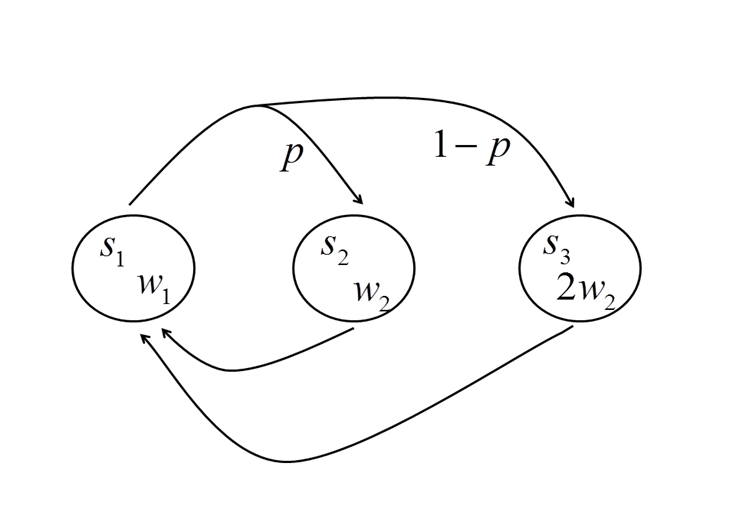
\includegraphics[width=0.6\textwidth]{hw8_a}
\end{center}

We consider a value function approximation $\tilde V(s) = {\phi _1}(s){w_1} + {\phi _2}(s){w_2}$, given explicitly as $\tilde V = {\left( {{w_1},{w_2},2{w_2}} \right)^ \top }$, and we let $w = {\left( {{w_1},{w_2}} \right)^ \top }$ denote the weight vector.

\begin{enumerate}
\setcounter{enumi}{1}
  \item What are the features $\phi (s)$ in this representation?
  \item Write down the Bellman operator ${T^\pi }$ explicitly. Write down${T^\pi }\tilde V$ .
  \item What is the stationary distribution?
  \item Write down the projection operator $\Pi $ explicitly, for $\epsilon = \left( \frac{1}{2},\frac{1}{4},\frac{1}{4}\right)$.
  \item Write an explicit expression for $\tilde V' \doteq \Pi {T^\pi }\tilde V$ in terms of $w$: the weight vector of $\tilde V$. Let $w' = {\left( {{w_1}',{w_2}'} \right)^ \top }$ denote the weights of $\tilde V'$. Write $w'$ as a function of $w$ .
  \item Show that iteratively applying $\Pi {T^\pi }$to $\tilde V$ may diverge for certain values of $p$.
\end{enumerate}
\end{exercise}

\begin{exercise}[\textbf{SARSA with function approximation}]
In this question we will implement a reinforcement learning algorithm in a continuous domain using function approximation.

Recall the tabular SARSA algorithm (Section \ref{ss:Q_eval}). We now present an extension of SARSA to the function approximation setting.
Assume that we are given a set of state-action features $\phi(s,a)\in \mathbb R^k$. We propose to approximate ${Q^\pi }(s,a)$ as a linear combination of these features:
$${\tilde Q^\pi }(s,a) = \mathop \sum \limits_{i = 1}^k {\phi _i}(s,a){w_i} \equiv \phi {(s,a)^ \top }w.$$
Our goal is to find the weight vector  $w \in \mathbb R^k$.

In the SARSA algorithm, at each stage we observe $\left( {{s_t},{a_t},{r_t},{s_{t + 1}},{a_{t + 1}}} \right)$, simulated on-policy (i.e., by simulating the policy $\pi $) and update $w$ by
\begin{align*}
w: &= w + {\beta _t}{\delta _t}\phi ({s_t},{a_t})\\
{\delta _t} &\buildrel \Delta \over = r({s_t}) + \gamma \phi {({s_{t + 1}},{a_{t + 1}})^ \top }w - \phi {({s_t},{a_t})^ \top }w
\end{align*}
where ${\beta _t}$ is a suitable step-size, and $\gamma $ is the discount factor.
\begin{enumerate}
  \item Explain the intuition for this update. You may use the TD(0) algorithm learned in class.
\end{enumerate}

Policy improvement in SARSA is achieved by choosing the policy $\pi $ as the  $\epsilon$-greedy policy with respect to the current $w$, that is, at time $t$ the state is ${x_t}$ and the action ${a_t}$ is selected according to
$${a_t} = \left\{ {\begin{array}{*{20}{c}}
{random}&{w.p.\,\,\,\epsilon}\\
{\arg {{\max }_a}\left( {\phi {{({s_t},a)}^ \top }w} \right)}&{w.p.\,\,1-\epsilon}
\end{array}} \right..$$

\begin{enumerate}
\setcounter{enumi}{1}
  \item Explain why the SARSA algorithm is expected to gradually improve performance.
\end{enumerate}

We will now implement SARSA on a popular RL benchmark - \emph{the mountain car}.
\begin{center}
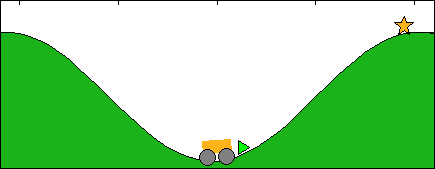
\includegraphics[width=0.6\textwidth]{hw8_b}
\end{center}

In the Mountain Car problem (see figure), an under-powered car must drive up a steep hill. Since gravity is stronger than the car's engine, even at full throttle, the car cannot simply accelerate up the steep slope. The car is situated in a valley and must learn to leverage potential energy by first driving up the left hill before gaining enough momentum to make it to the goal at the top of the right hill.

The state space is two-dimensional, and consists of the position $p \in \left[ { - 1.2,0.6} \right]$ and velocity $v \in \left[ { - 0.07,0.07} \right]$. There are 3 actions: $a =  - 1$ (accelerate left), $a = 0$ (don't accelerate), and $a = 1$ (accelerate right).

The simulation runs in episodes. At the beginning of an episode the initial state is ${p_0}\sim Uniform\left[ { - 0.5,0.2} \right]$, ${v_0}\sim Uniform\left[ { - 0.02,0.02} \right]$. If the car reaches the right hilltop: $p > 0.5$, the episode ends, and a reward $r = 5$ is received. At every other step the reward is $r =  - 1$. The maximum episode length is 500 steps.

The Matlab function \texttt{mountainCarSim(p, v, u)} (available at the course webpage) takes the current state and action and returns the next state of the car.

As function approximation, we will use grid-tiles. For each action $a$, we discretize the state space into $n$ non-overlapping tiles of size ${\Delta _p} = 0.1,{\Delta _v} = 0.01$ (see figure), and we label the tiles $\psi _1^a, \ldots ,\psi _n^a$.
\begin{center}
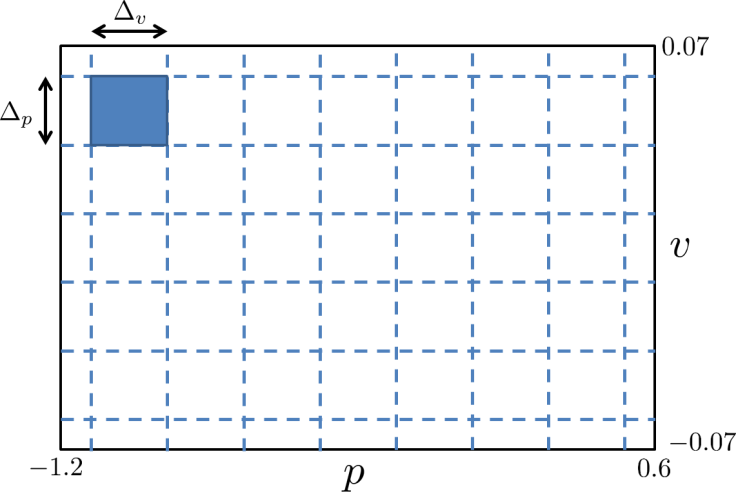
\includegraphics[width=0.6\textwidth]{hw8_c}
\end{center}

Define binary \textbf{state-features} $\phi(s)\in \mathbb R^n$  by:
\[{\phi _i}(s) = \left\{ {\begin{array}{*{20}{c}}
1&{s \in {\psi _i}\,}\\
0&{else}
\end{array}} \right.,\]
and binary \textbf{state-action-features} $\phi(s,a)\in \mathbb R^k$  where $k = 3n$,  by:
\[\begin{array}{l}
\phi (s, - 1) = \left\{ {\phi (s),2n\,\,{\rm{zeros}}} \right\}\\
\phi (s,0) = \left\{ {n\,\,{\rm{zeros}},\phi (s),n\,\,{\rm{zeros}}} \right\}\\
\phi (s,1) = \left\{ {2n\,\,{\rm{zeros}},\phi (s)} \right\}
\end{array}.\]

\begin{enumerate}
\setcounter{enumi}{2}
  \item Run the SARSA algorithm in this domain. Generate the following plots, and write a proper explanation for each plot.
  \begin{enumerate}
    \item Total reward (in episode) vs. episode
    \item Goal was reached / not reached vs. episode
    \item ${L_2}$ Norm of the weights $w$ vs. episode
    \item Trajectory of car ($p$ vs. time) for the greedy policy starting from $\left( {0,0} \right)$, every 100 episodes of learning.
    \item Final value function and policy after learning.
  \end{enumerate}
\end{enumerate}

You may use the following learning parameters for the algorithm:
\begin{itemize}
  \item Step size: ${\beta _t} = \frac{{100}}{{1000 + {\rm{episode count}}}}$
  \item Exploration: $\epsilon = 0.1$
  \item Discount: $\gamma  = 0.95$
  \item Total number of learning episodes: $500 - 1000$
  \item Initial weights: zeros.
\end{itemize}

\paragraph{Bonus:} Improve the learning algorithm using either:
\begin{itemize}
  \item Different features - you may try:
  \begin{itemize}
    \item Overlapping tiles (sometime called CMACs) (\url{http://webdocs.cs.ualberta.ca/~sutton/book/ebook/node88.html#SECTION04232000000000000000})
    \item Radial Basis Functions (\url{http://en.wikipedia.org/wiki/Radial_basis_function})
    \item Fourier / polynomials (\url{http://irl.cs.duke.edu/fb.php})
  \end{itemize}
  \item Different algorithm - you may try:
  \begin{itemize}
    \item SARSA($\lambda $) e.g., \url{http://webdocs.cs.ualberta.ca/~sutton/book/ebook/node89.html}
    \item Q($\lambda $) e.g., \url{http://webdocs.cs.ualberta.ca/~sutton/book/ebook/node89.html}
  \end{itemize}
  \item Any other idea that you like
\end{itemize}
Evidence that your method improves performance in some sense (learning rate/ final performance/ robustness to parameter changes/ etc.) will be rewarded with bonus points.
\end{exercise} 